\documentclass[a4paper]{article}
\usepackage[utf8x]{inputenc}
\usepackage[T1,T2A]{fontenc}
\usepackage[russian]{babel}
\usepackage{hyperref}
\usepackage{indentfirst}
\usepackage{listings}
\usepackage{color}
\usepackage{here}
\usepackage{array}
\usepackage{multirow}
\usepackage{graphicx}
\usepackage{caption}
\graphicspath{{graphics/}}
\usepackage[left=2cm,right=2cm,
top=2cm,bottom=2cm,bindingoffset=0cm]{geometry}
\usepackage{listings}
\lstset{ %
	extendedchars=\true,
	keepspaces=true,
	language=bash,					% choose the language of the code
	basicstyle=\footnotesize,		% the size of the fonts that are used for the code
	numbers=left,					% where to put the line-numbers
	numberstyle=\footnotesize,		% the size of the fonts that are used for the line-numbers
	stepnumber=1,					% the step between two line-numbers. If it is 1 each line will be numbered
	numbersep=5pt,					% how far the line-numbers are from the code
	backgroundcolor=\color{white},	% choose the background color. You must add \usepackage{color}
	showspaces=false				% show spaces adding particular underscores
	showstringspaces=false,			% underline spaces within strings
	showtabs=false,					% show tabs within strings adding particular underscores
	frame=single,           		% adds a frame around the code
	tabsize=2,						% sets default tabsize to 2 spaces
	captionpos=b,					% sets the caption-position to bottom
	breaklines=true,				% sets automatic line breaking
	breakatwhitespace=false,		% sets if automatic breaks should only happen at whitespace
	escapeinside={\%*}{*)},			% if you want to add a comment within your code
	postbreak=\raisebox{0ex}[0ex][0ex]{\ensuremath{\color{red}\hookrightarrow\space}}
}

\begin{document}	% начало документа

\begin{titlepage}	% начало титульной страницы

	\begin{center}		% выравнивание по центру

		\large Санкт-Петербургский Политехнический Университет Петра Великого\\
		\large Институт компьютерных наук и технологий \\
		\large Кафедра компьютерных систем и программных технологий\\[6cm]
		% название института, затем отступ 6см
		
		\huge Телекоммуникационные технологии\\[0.5cm] % название работы, затем отступ 0,5см
		\large Отчет по лабораторной работе №1 \\[0.1cm]
		\large\textbf{"Сигналы телекоммуникационных систем"}\\[5cm]

	\end{center}


	\begin{flushright} % выравнивание по правому краю
		\begin{minipage}{0.25\textwidth} % врезка в половину ширины текста
			\begin{flushleft} % выровнять её содержимое по левому краю

				\large\textbf{Работу выполнила:}\\
				\large Власова А.В.\\
				\large {Группа:} 33501/4\\
				
				\large \textbf{Преподаватель:}\\
				\large Богач Н.В.\

			\end{flushleft}
		\end{minipage}
	\end{flushright}
	
	\vfill % заполнить всё доступное ниже пространство

	\begin{center}
	\large Санкт-Петербург\\
	\large \the\year % вывести дату
	\end{center} % закончить выравнивание по центру

\thispagestyle{empty} % не нумеровать страницу
\end{titlepage} % конец титульной страницы

\vfill % заполнить всё доступное ниже пространство

\section{Цель работы}
Познакомиться со средствами генерации и визуализации простых сигналов.

\section{Постановка задачи}
В командном окне MATLAB и в среде Simulink промоделировать синусоидальный и прямоугольный сигналы с различными параметрами. Получить их спектры. Вывести на график.

\section{Теоретический раздел}
Сигнал — носитель информации, используемый для передачи сообщений в системе связи. Сигналом может быть любой физический процесс, параметры которого изменяются (или находятся) в соответствии с передаваемым сообщением. Сигнал, детерминированный или случайный, описывают математической моделью, функцией, характеризующей изменение параметров сигнала. Математическая модель представления сигнала, как функции времени, является основополагающей концепцией теоретической радиотехники, оказавшейся плодотворной как для анализа, так и для синтеза радиотехнических устройств и систем.\\\\
Спектр сигнала — результат разложения сигнала на более простые в базисе ортогональных функций. В радиотехнике в качестве базисных используют синусоидальные функции. Разложение сигнала обычно проводят с помощью преобразования Фурье.\\\\
Всякая периодическая функция $y(t)$, удовлетворяющая условиям Дирихле, может быть представлена в виде ряда Фурье:\\

$y(t) = \sum_{k=-\infty}^{\infty}C_ke^{j2{\pi}kft}$\\

где $f = \frac{1}{T}$, $T$ -- период функции $y(t)$, $C_k$ -- постоянные коэффициенты. Условия Дирихле означают, что функция должна быть ограниченной, кусочно-непрерывной и иметь на протяжении периода конечное число экстремумов.\\

В качестве базовых функций использованы комплексные гармонические функции вида $e^{j2{\pi}kft}$, где $k$ -- целочисленный параметр. Наряду с комплексными гармониками в качестве базисных могут использоваться вещественные гармонические функции $sin(2{\pi}kft)$ и $cos(2{\pi}kft)$. Более того, в общенном ряде Фурье возможно использование любых базовых ортогональных функций.\\

Значения коэффициентов $C_k$ ряда Фурье находятся по формуле:\\

$C_k = \frac{1}{T}\int_{t_0}^{t_0+T}y(t)e^{-j2{\pi}kft}dt$\\

\section{Ход работы}
\subsection{Моделирование в Matlab}

В командном окне Matlab промоделируем синусоидальные сигналы с разными параметрами и найдем их спектры. 

\captionof{lstlisting}{Генерация синусоидального сигнала}
\lstinputlisting{../sinusoidal.m}

\begin{center}
	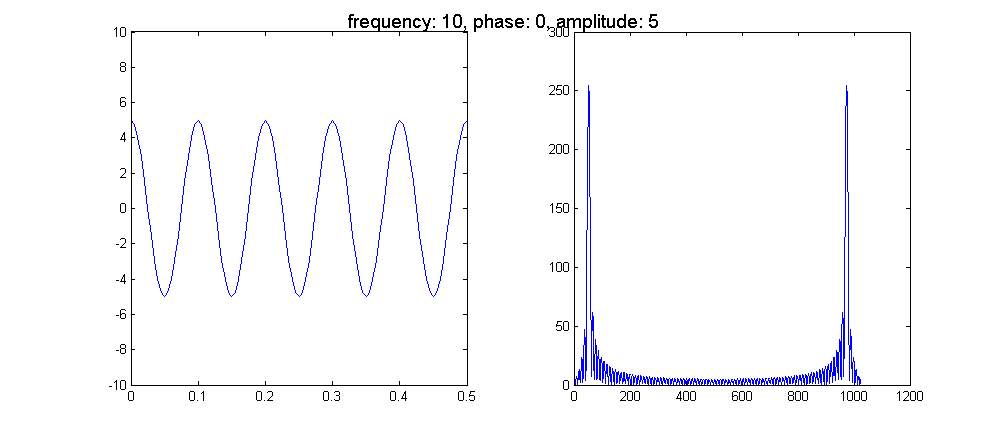
\includegraphics[scale = 0.5]{sin1.png}
	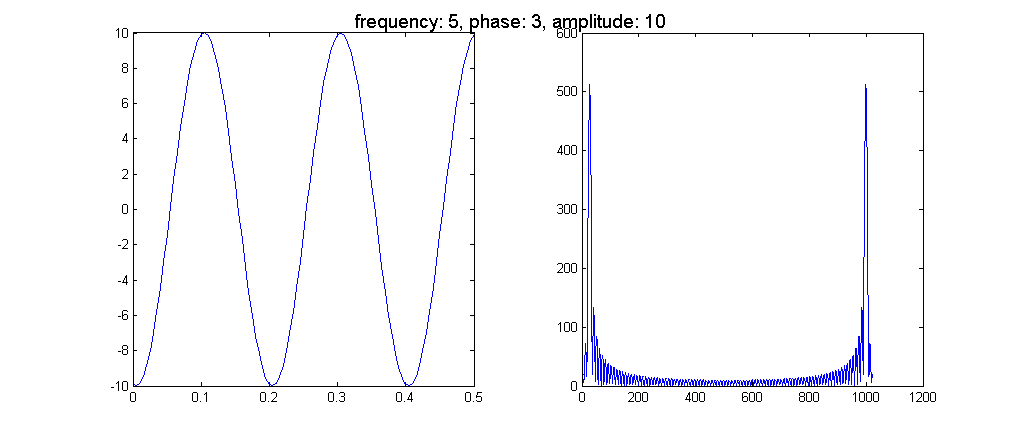
\includegraphics[scale = 0.5]{sin2.png}
	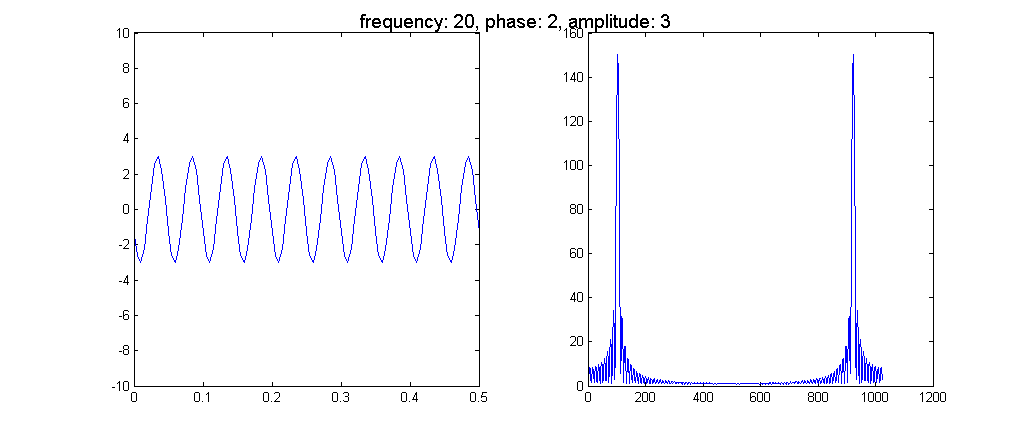
\includegraphics[scale = 0.5]{sin3.png} \\ Рис.1 Синусоидальные сигналы и их спектры 
\end{center} 

\newpage

Сгенерируем прямоугольные сигналы и найдем их спектры.

\captionof{lstlisting}{Генерация прямоугольного сигнала}
\lstinputlisting{../meander.m}

\begin{center}
	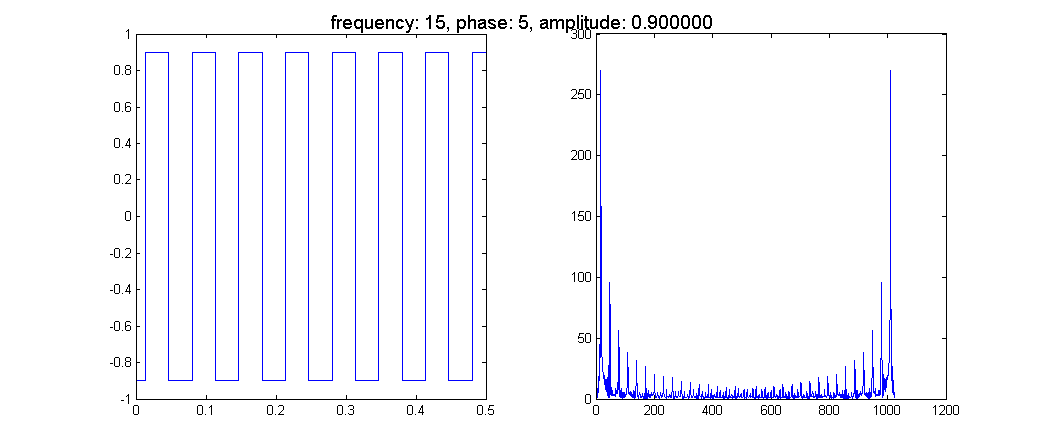
\includegraphics[scale = 0.5]{square1.png}
	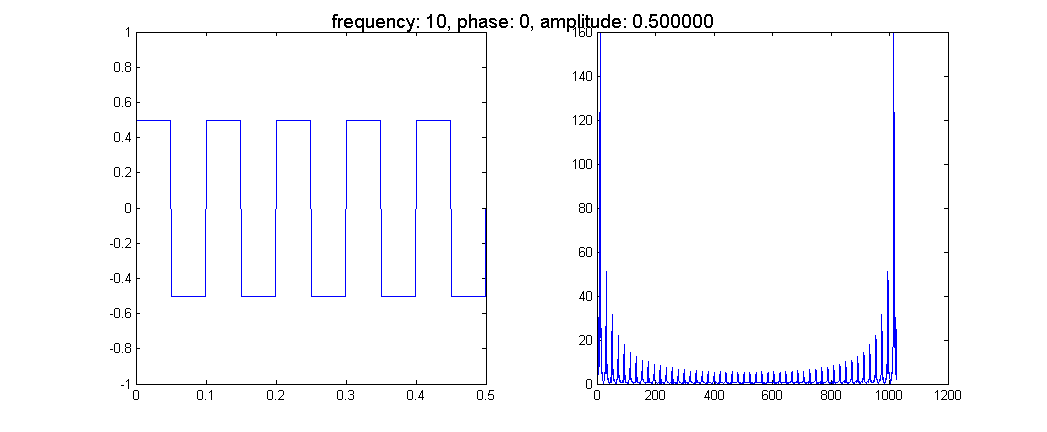
\includegraphics[scale = 0.5]{square2.png}
	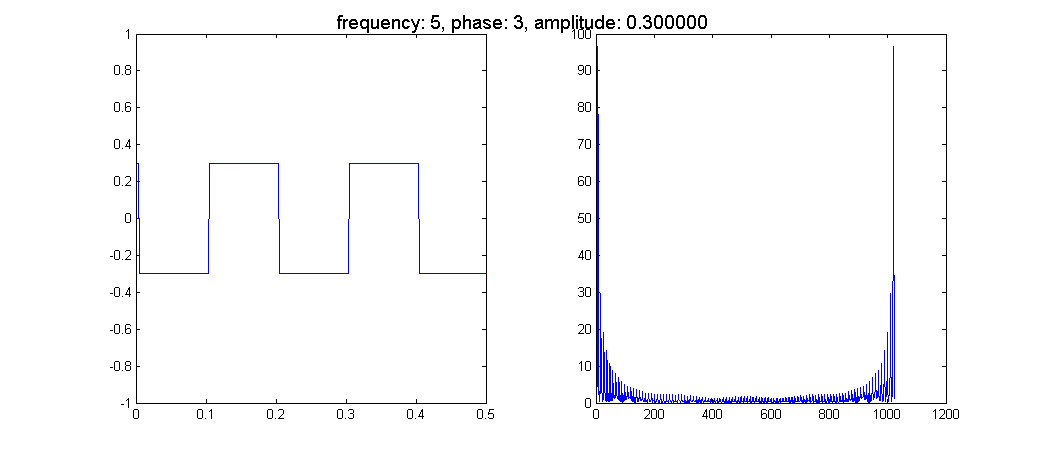
\includegraphics[scale = 0.5]{square3.png} \\ Рис.2 Прямоугольные сигналы и их спектры 
\end{center}

\subsection{Моделирование в Simulink}

В среде Simulink промоделируем синусоидальный сигнал.

\center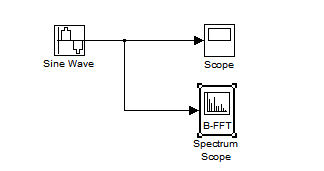
\includegraphics[scale = 1]{scheme1.png} \\ Рис. 3 Схема для исследования синусоидального сигнала \\

~\
\flushleft Исследуем сигнал с частотой 10 рад/с.
\center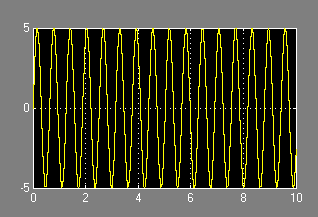
\includegraphics[scale = 1]{sin_sim1.png} \\ Рис. 4 Сигнал с частотой 10 рад/с \\ 
\center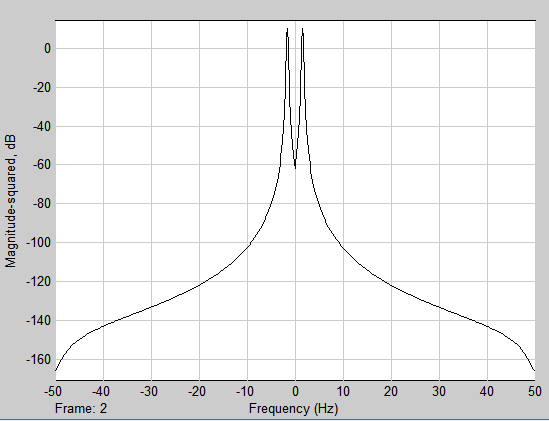
\includegraphics[scale = 0.7]{sin_sim_spectrum1.png} \\ Рис.5 Спектр сигнала \\

~\
\flushleft Изменим частоту сигнала на 2 рад/с.
\center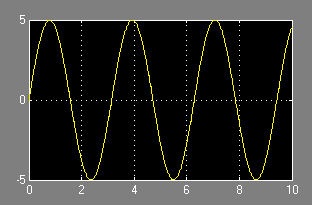
\includegraphics[scale = 1]{sin_sim2.png} \\ Рис. 6 Сигнал с частотой 2 рад/с \\ 
\center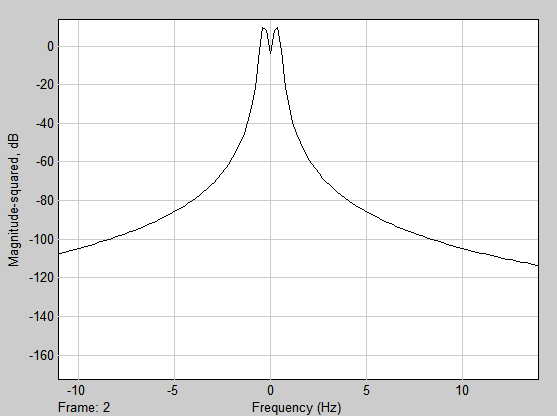
\includegraphics[scale = 0.7]{sin_sim_spectrum2.png} \\ Рис.5 Спектр сигнала \\

~\
\flushleft Создадим схему для исследования прямоугольных сигналов.
\center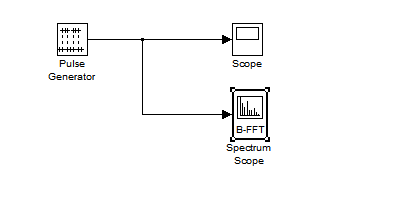
\includegraphics[scale = 1]{scheme2.png} \\ Рис. 7 Схема для исследования прямоугольного сигнала \\

~\
\flushleft Исследуем сигнал с частотой 5 Гц.
\center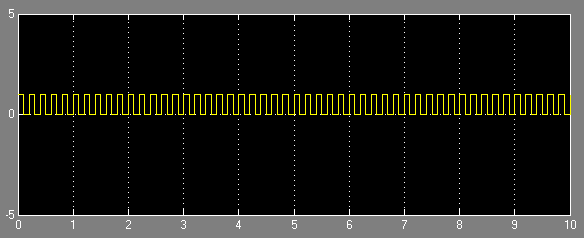
\includegraphics[scale = 0.8]{square_sim1.png} \\ Рис. 8 Прямоугольный сигнал с частотой 5 Гц \\ 
\center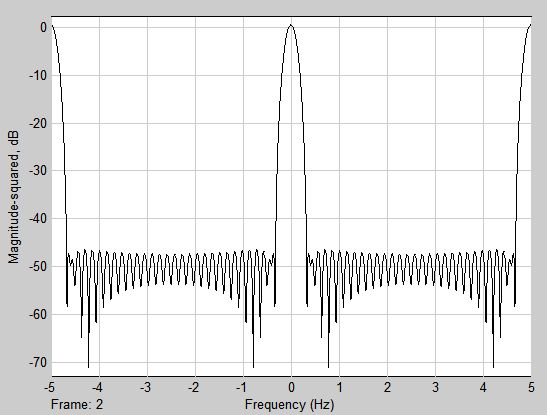
\includegraphics[scale = 0.7]{square_sp1.png} \\ Рис. 9 Спектр сигнала \\

~\
\flushleft Уменьшим частоту сигнала в 2 раза.
\center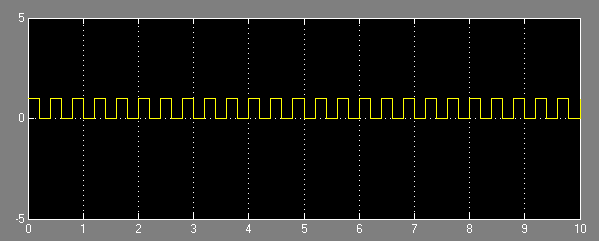
\includegraphics[scale = 0.8]{square_sim2.png} \\ Рис. 10 Сигнал с частотой 2.5 Гц \\ 
\center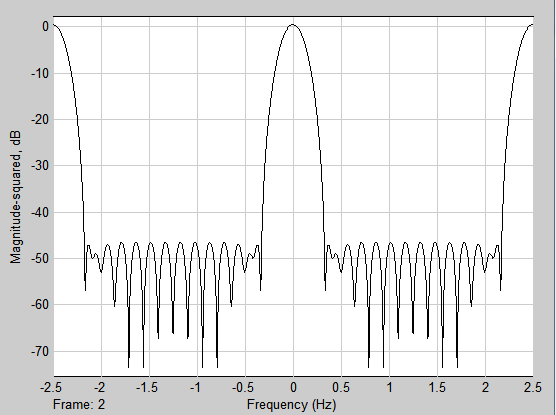
\includegraphics[scale = 0.7]{square_sp2.png} \\ Рис.11 Спектр сигнала \\

\flushleft \section{Выводы}
В ходе выполнения лабораторной работы получены навыки использования средств генерации и визуализации простых сигналов в Matlab и Simulink.\\

Одним из признаков классификации сигналов является способ его задания. Существуют регулярные (детерминированные) и нерегулярные (случайные) сигналы. Детерминированные сигналы задаются аналитической функцией, а случайные принимают произвольные значения в каждый момент времени.\\

Также сигналы классифицируют в зависимости от функций, которые описывают их параметры. Выделяют следующие сигналы:
\begin{itemize}
	\item аналоговые сигналы, описываемые непрерывной функцией;
	\item дискретные сигналы, описываемые функцией взятых в определенные моменты времени отсчетов;
	\item сигналы, квантованные по уровню;
	\item цифровые сигналы (дискретные и квантованные по уровню).
\end{itemize}
\end{document}






